\documentclass{prova}

\usepackage{amsmath}
\usepackage{amsfonts}

\setlength{\textheight}{25cm}

\renewcommand{\sin}{\,\mbox{sen}\,}
\newcommand{\ds}{\displaystyle}

\professor{Prof.\@ Adriano Barbosa}
\disciplina{C\'alculo de V\'arias Vari\'aveis}
\avaliacao{P1}
\curso{Matem\'atica}
\data{13/02/2023}

\begin{document}
	\cabecalho{5}  % o numero 5 indica a qnt de quadros na tabela de nota

    \textbf{Todas as respostas devem ser justificadas.}

    \begin{questionario}
        \q{Determine e esboce o dom\'{\i}nio de $F(x,y)=1+\sqrt{4-y^2}$.}
        \q{Determine o sinal das derivadas parciais de $f(x,y)=x^2-xy$ em:}

            \begin{minipage}{0.6\textwidth}
                \begin{questionario}
                    \qq{$P=(1,0).$}
                    \qq{$Q=(0,1).$}
                    \qq{No ponto $A$ justificando sua resposta.}
                    \qq{No ponto $B$ justificando sua resposta.}
                \end{questionario}
            \end{minipage}
            \begin{minipage}{0.4\textwidth}
                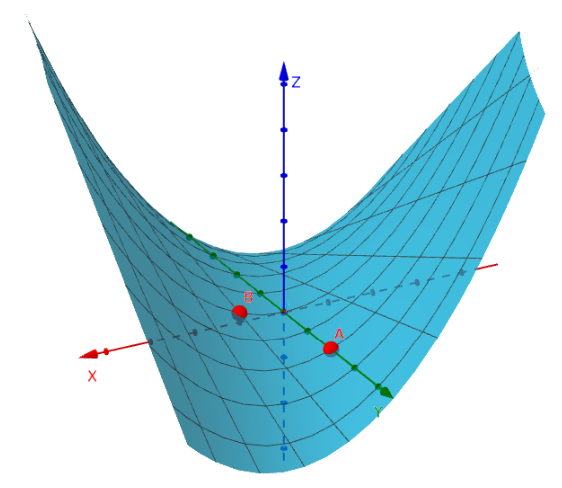
\includegraphics[width=\textwidth]{fig1.png}
            \end{minipage}
        \q{Se $z=f(x-y)$, mostre que $\ds\frac{\partial z}{\partial
           x}+\frac{\partial z}{\partial y}=0$.}
        \q{A temperatura $T$ de um ponto $P$ numa bola de metal \'e inversamente
           proporcional \`a dist\^ancia de $P$ ao centro da bola, que tomamos como
           sendo a origem. A temperatura no ponto $(1,2,2)$ \'e de $120^{\circ}$C.
           Determine a taxa de varia\c{c}\~ao de $T$ em $(1,2,2)$ na dire\c{c}\~ao
           $(1,-1,1)$.}
        \q{Determine os m\'aximos e m\'{\i}nimos de $f(x,y,z)=2x+2y+z$ restrita a
           $x^2+y^2+z^2=9$.}
        \q{(B\^onus) Uma fun\c{c}\~ao $f$ \'e chamada homog\^enea de $n$-\'esimo grau se satisfaz a
           equa\c{c}\~ao $f(tx,ty)=t^n f(x,y)$ para todo $t$, onde $n$ \'e um inteiro
           positivo e $f$ tem derivadas parciais de segunda ordem cont\'{\i}nuas.}
           \begin{questionario}
                \qq{Verifique se $f(x,y)=x^2y+2xy^2+5y^3$ \'e homog\^enea de grau
                    3.}
                \qq{Mostre que, se $f$ \'e homog\^enea de grau $n$, ent\~ao}
                    \[x\frac{\partial f}{\partial x} + y\frac{\partial
                      f}{\partial y} = nf(x,y)\]
                      [Dica: utilize a regra da cadeia para derivar $f(tx,ty)$
                       com rela\c{c}\~ao a $t$.]
           \end{questionario}
    \end{questionario}
\end{document}
